


%----------------------------------------------------------------------------------------------------%
\begin{frame}
\frametitle{Functions and Definite integrals}
\begin{itemize}
\item Integration is not part of the syllabus, and it is assumed that students are not familiar with how to compute definite integrals.
\item However,  it is useful to know what the purpose of definite integrals are, because we will be using the results derived from definite integrals. \item It is assumed that students are familiar with functions.
\end{itemize}
\end{frame}
%----------------------------------------------------------------------------------------------------%
\begin{frame}
\frametitle{Functions}

\vspace{-0.5cm}

\begin{center}
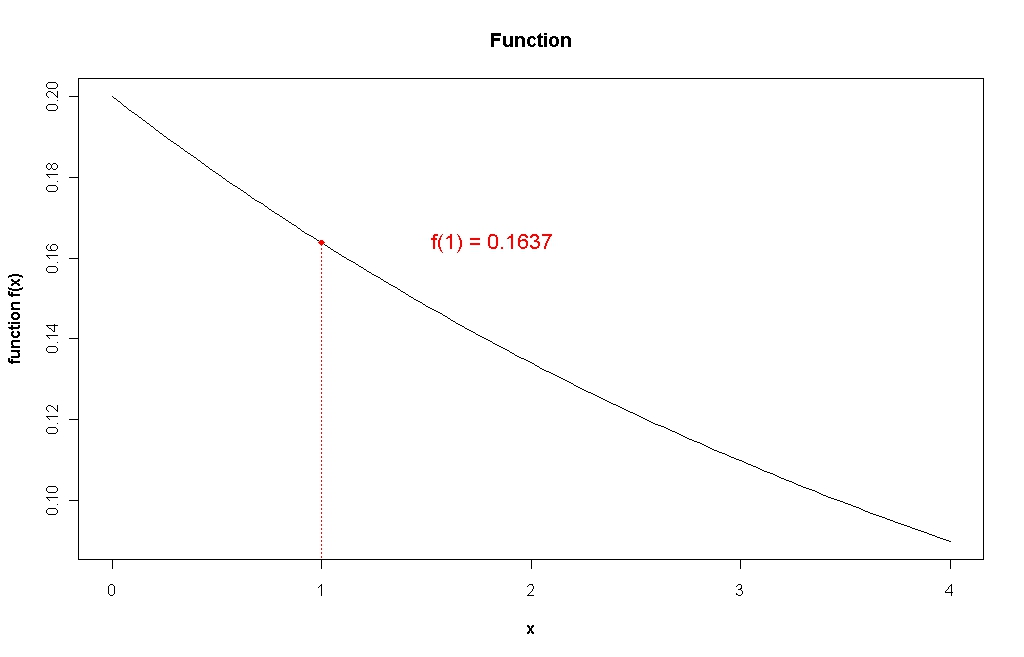
\includegraphics[scale=0.30]{images/6AFunction}

\end{center}

Some function $f(x)$ evaluated at $x=1$.
\end{frame}





%----------------------------------------------------------------------------------------------------%
\begin{frame}
\frametitle{Cumulative Distribution Function}

\vspace{-0.5cm}
\begin{center}
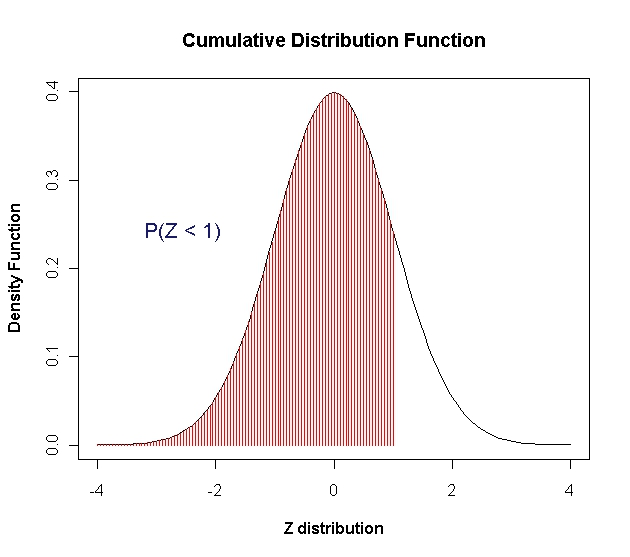
\includegraphics[scale=0.35]{images/6ACDF}

\end{center}
Cumulative Distribution Function $P(Z \leq 1)$.
\end{frame}


\end{documents}



%----------------------------------------------------------------------------------------------------%
\begin{frame}
\frametitle{Cumulative Distribution Function}
\vspace{-0.5cm}
\begin{center}
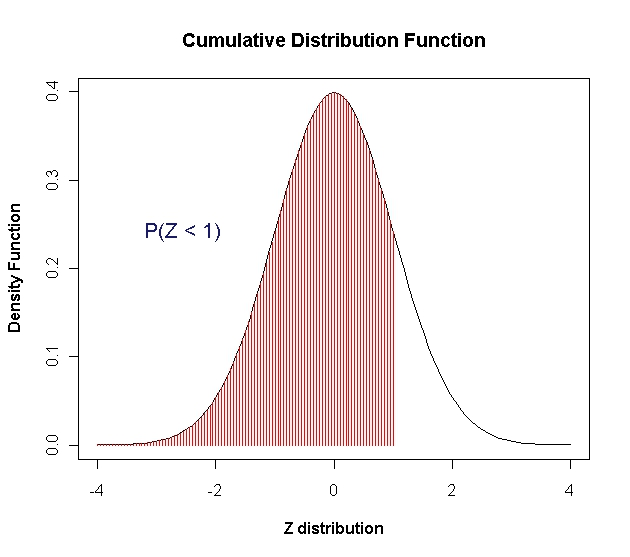
\includegraphics[scale=0.35]{images/6ACDF}
\end{center}
Cumulative Distribution Function $P(Z \leq 1)$ \\ Here the random variable is called $Z$ (we will see why later)
\end{frame}


%----------------------------------------------------------------------------------------------------%
\frame{
\frametitle{The Cumulative Distribution Function }
Recall:
\begin{itemize}
\item The \textbf{\emph{cumulative distribution function}} (CDF), (or just distribution function), describes the probability that a continuous random variable X with a given probability distribution will be found at a value less than or equal to x.\\

\[ F_X(x) = P(X \leq x) \]

\item Intuitively, it is the ``area so far" function of the probability distribution.
\end{itemize}
}


%----------------------------------------------------------------------------------------------------%
\frame{
\frametitle{The Cumulative Distribution Function }
The cumulative distribution function (CDF), or just distribution function, describes the probability that a real-valued random variable X with a given probability distribution will be found at a value less than or equal to x.\\ Intuitively, it is the ``area so far" function of the probability distribution. 

\[ F_X(x) = P(X \leq x) \]
}

%------------------------------------------------------------------%
\frame{
\frametitle{Exact Probability}
\large
\alert{Remarks:} This is for continuous distributions only.
\begin{itemize}
\item The probability that a continuous random variable will take an exact value is infinitely small.
We will usually treat it as if it was zero.
\item
When we write probabilities for continuous random variables in mathematical notation, we often retain the equality component (i.e. the "...or equal to..").\\
For example, we would write expressions $P(X \leq 2)$ or $P(X \geq 5)$.
\item
Because the probability of an exact value is almost zero, these two expression are equivalent to $P(X < 2)$
or $P(X > 5)$. \item The complement of $P(X \geq k)$ can be written as $P(X \leq k)$.
\end{itemize}
}


%------------------------------------------------------------------%




